\ifx\master\undefined\input{settings/autocompile}\fi
%
\chapter*{Conclusion}
\addcontentsline{toc}{chapter}{Conclusion}
\label{ch:conclusions}

This thesis has presented a search for MSSM Higgs bosons in the 2010 7~\TeV
CMS data set. Two new experimental methods, the TaNC tau identification
algorithm, and the SVfit mass reconstruction method have been introduced in this
thesis.  Both methods increased the sensitivity of the search.  The search
was performed using 36~\pbinv of data.  The expected event yield from standard
model sources is 577 events. In total, 573 events were selected; the observed is
compatible with the standard model.  No signal--like excess of events is
observed.  We set an upper limit on the production of Higgs bosons, and
interpret this limit in the context of the MSSM.

The analysis presented in this thesis was part of a larger
study~\cite{HIG-10-002} performed by the CMS collaboration searching for the
MSSM Higgs boson decaying to tau leptons.  The CMS analysis used three channels,
the $H \to \tau \tau \to e\tau_h$, $H \to \tau \tau \to e\mu$, and the
$\mu\tau_h$ channel.  The $\mu\tau_h$ channel search presented in this thesis
is very similar to the CMS result.  While not as pure as the $\mu\tau$ channel,
the inclusion of the high--statistics $e-\tau$ channel increases the sensitivity
of the CMS analysis.  The $e\mu$ channel has low statistics, but is not
sensitive to the systematic uncertainty on the hadronic tau identification.  The
region of the MSSM parameter space excluded by combined CMS result is
illustrated in Figure~\ref{fig:CMSTanBetaExclusionWTF}.  At the time of this
writing, the CMS result described in~\cite{HIG-10-002} sets the most stringent
limits on the MSSM using a direct search.  
%
\begin{figure}[htb]
  \centering
  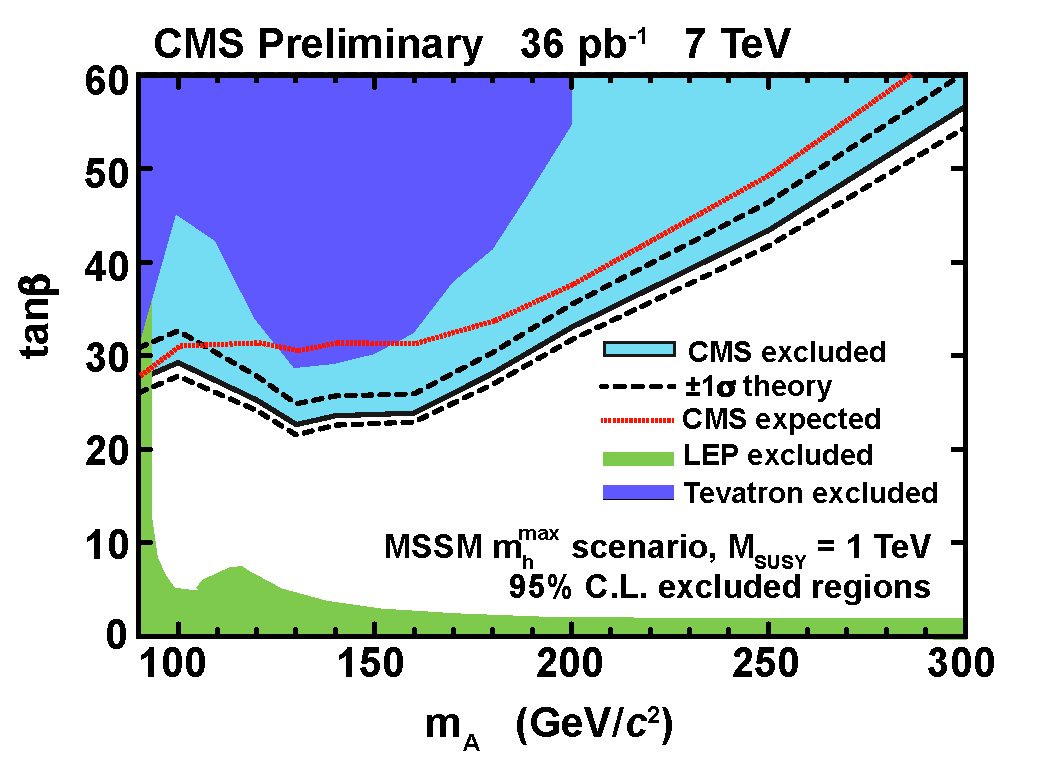
\includegraphics[width=\textwidth]{conclusions_chapter/figures/tanbeta-ma-LEP-Tev.pdf}
  \caption[CMS combined exclusion of MSSM $\tb-\ma$ parameter space]{Region of MSSM
  $\tb-\ma$ parameter space excluded by the CMS combined
  analysis~\cite{HIG-10-002}.}
  \label{fig:CMSTanBetaExclusionWTF} 
\end{figure}

\ifx\master\undefined\input{settings/autocompile}\fi
